\documentclass[12pt,a4paper]{article}

\usepackage[utf8]{inputenc}
\usepackage{amsmath}
\usepackage{amsfonts}
\usepackage{amssymb}
\usepackage{tabularx}
\usepackage{graphicx}

%font
\usepackage[T1]{fontenc}
\usepackage{uarial}
\renewcommand*{\familydefault}{\sfdefault}


\author{Bardia Jedi}
\title{Personing Brev SoftwareEng}
\begin{document}
	\makebox[0pt][l]{%
 	\raisebox{-\totalheight}[0pt][0pt]{%
    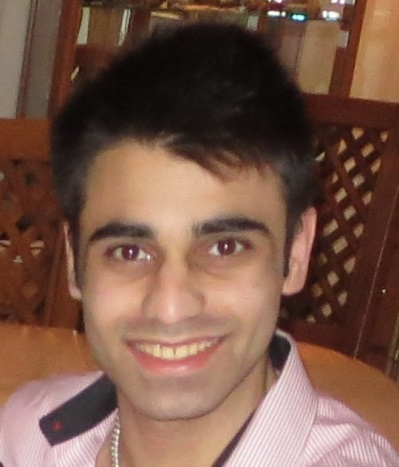
\includegraphics[width=30mm]{pimg01.jpg}}}%
	
	
	\begin{tabularx}{ \textwidth}{ l X r  }				
  		 			&& 
  			\begin{tabular}{ r  l }
					& \textbf{Bardia Jedi}\\
					& Kakelösagatan 3\\
					& 43144 MÖLNDAL\\			
  					& 0768-957983\\
  					& bardiajedi@gmail.com \\
 
			\end{tabular}\\
	\end{tabularx}
	\vspace{12pt}

	%uniqe
	\begin{flushleft}
		\setlength{\parindent}{2ex}
		
			
		
		\hspace{1.5ex}
		När det handla om dator jag de folk vill ha!
		%\vspace{24pt}
		%\hspace{6pt}
		
	Jag har varit ett sfotwera enginerings student, och med mig jag hämtar goda kunskaper om telekommunikation och Object Oriented språk (java, c++, c\# och mycket mera).

	Allting från installation till maintenance/ diagnostics kommer med mig också. Om det är något jag saknar i mitt kit, är jag väl förberedd att lära mig att lära mig det.
	
	
	Programvaror design är var jag lyser som bäst. 
	Fast jag har litet att visa inom det eftersom jag inte har jobbat kommersiellt.
	Mest av mina har varit för eget komfort, som exmaple jag har gjort rss reader, html table extractor, en encryption system med en enkel gui, a log reader with gui, jag håller på att göra en sudoku spel med analys motor, och min första projekt var ett randomstion motor till ett spel jag spelar, den är special eftersom den visa en del av vad jag kan göra både from grafik och programmering design, den har lilla appen är enkel customiser både via xml och mjukvara generation. 
	Om ni är intresserade konkat mig och jag kommer skickar er source-en och och executable-en.
	
	
	Som ni vet jag har ingen arbeteserfarenhet fäst jag har en hel del egna erfarenhet.
	
	\hspace{6pt}
	Jag är alltid redo för ny utmaningar och om att lära sig nya saker jag har en villa för ny kunskap. 

 
	 
	 	

	\end{flushleft}
		
	\newpage
	
	%shared
	\begin{flushleft}
	\setlength{\parindent}{2ex}	
			\hspace{2ex}
			Hej Jag heter Bardia Jedi.	
			Jag är född den 10 okt 1991 i Tehran/Iran och emigrerade till Sverige 2004. 
			Som person är jag social, engagerad och är en ordningsam kille som alltid vill bli	bättre på det jag gör. 
			Dessutom kommer jag alltid i tid och är pålitlig.
\vspace{12pt}

			Jag är en ”open minded” person och som mål ger jag alltid 100 \% av det jag kan, och 110 \% om jag behöver komma i kapp. 
			Med vänner/kollegor är jag alltid vänlig och har en ömsesidig relation och jag försöker alltid att ha en professionell relation med de jag jobbar med.
			\vspace{12pt}

		Mitt mål i arbetslivet är tre enkla ord, nämligen att lära, behärska och imponera.
		
		\vspace{12pt}		
		\noindent 
		Med det menar jag:\\
		\noindent		
		Lär hur mycket du kan. Lär mycket mera. Visa ett lyssnade resultat.
		\vspace{24pt}
		
		\noindent
		Mvh/ Bardia Jedi
	\end{flushleft}
	
	
	
\end{document}